\section{Problem identifikacije penjačkih smjerova i ograničenja tradictionalnih alata}

Tradicionalno, glavni izvor informacija za penjače su tiskani penjački vodiči. Ovi vodiči sadrže detaljne opise penjališta, karte pristupa, kao i skicirane prikaze stijene ili često nazivane \textit{topo} s ocrtanim linijama penjačkih smjerova, njihovim nazivima i težinama. Iako su desetljećima bili nezamjenjiv alat, tiskani vodiči imaju ograničenja. Podložni su zastarijevanju jer ne mogu pratiti dinamiku promjena na penjalištima poput dodavanja novih smjerova, promjena težina ili upozorenja o opasnostima na pojedinim smjerovima. Bilo kakve promjene zahtjevaju novo tiskanje i kupovanje novog izdanja. Tiskani vodiči su nepraktični za nošenje, a najveći izazov predstavlja interpretacija dvodimenzionalnih skica, koje su često slikane iz daljine, na trodimenzionalnu strukturu stijene. Proces lociranja točnog početka smjera na temelju crteža često je subjektivan, dugotrajan i može dovesti do frustracija ili pokušaj penjanja smjera koji je težinski izvan dohvata za penjača. 

\begin{figure}[H]
    \centering
    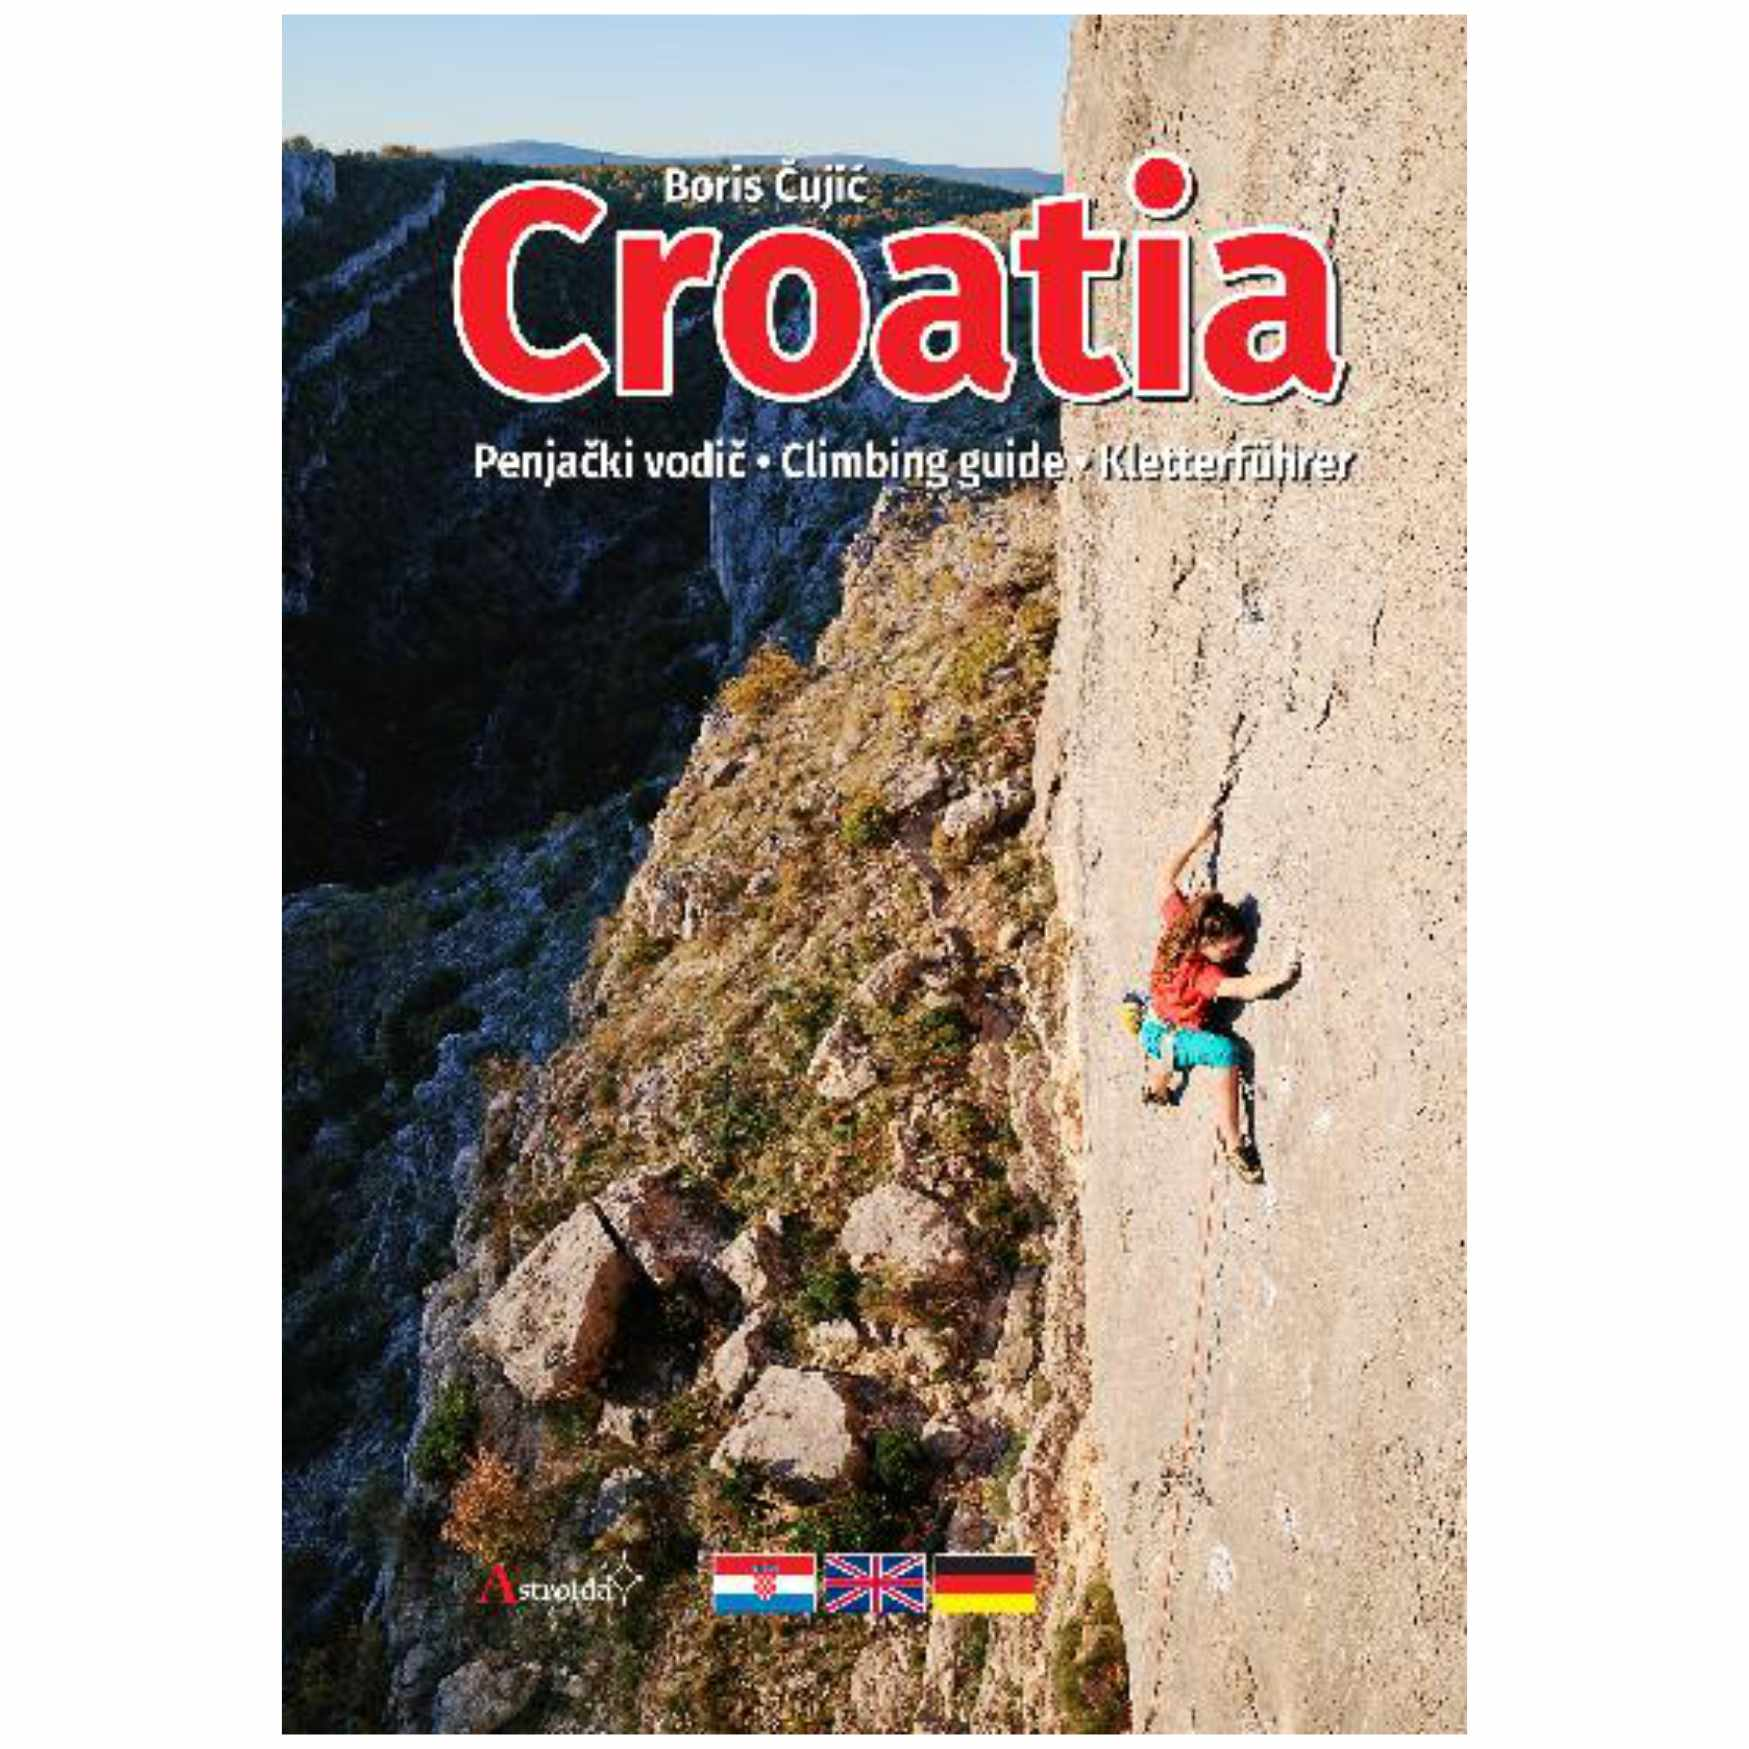
\includegraphics[width=0.8\textwidth]{images/uvod/tradicionalni_vodic.jpg}
    \caption{Prikaz tiskanog penjačkog vodiča}
\end{figure} 